\documentclass[../../monografia.tex]{subfiles}
\graphicspath{ {images/}{../images/}{../../images/}{../../../images/} }

\begin{document}

\section{Test Setup}
\label{section: Test Setup}

As the main project is a simulation, the best way to validate the project was to create the same situation that was created in the simulation in real life. With that, it could compare the performance in the simulated environment with a similar real-life situation.

For it, we choose to use the Pioneer 2 DX \cite{pioneer2dx_2024}, the same robot that we used in the simulation, but as your simulation has not good support for communication protocols and PWM, we had to add one adapter between the information from the real robot and the bluepill.

In general, the Pioneer 2 DX adapter is responsible for getting all the information from the robot by communication protocol and sending it to the bluepill in the form of digital values with GPIOS. In contrast, the Pioneer 2 DX adapter is also responsible for getting velocity from each motor that the bluepill has sent and sending it back to pioneer 2DX.

It is possible to visualize the general schema in the figure \ref{fig: Test Setup - General}.

%---
\begin{figure}[h]
    \centering
    \caption{Test Setup - General}
    \centering % para centralizarmos a figura
    \includegraphics[width=16cm]{diagramas-test_setup-general.drawio.png}
    \label{fig: Test Setup - General}
\end{figure}
%---

\subsection{Hardware}

The hardware of the project has two main functionality:

\begin{itemize}
    \item {Connect the ESP32 D1 Mini with the bluepill}
    \item {Connect the ESP32 D1 Mini with the pioneer 2DX}
\end{itemize}

The connection between the Bluepill and the ESP32 is detailed in Table \ref{table: Connection between Esp32 and Bluepill}. A transistor is placed between the rst\_signal from the Bluepill and the ESP32 D1 Mini. This enables the ESP32 to be reset manually and ensures the signal stays high even when the Bluepill’s signal is low.

It is possible to check the whole developed pcb for this interface in our github repository in our organization \cite{pioneer_2dx_interface_pcb_2024}.

\begin{table}[h!]
\caption{Connection between Esp32 and Bluepill}
\begin{tabular}{|l|l|l|l|l|l|l|}
\cline{1-3} \cline{5-7}
Label       & Bluepill Pin & ESP32 Pin &  & Label         & Bluepill Pin & ESP32 Pin \\ \cline{1-3} \cline{5-7} 
DD1         & PA4          & SD3       &  & encoder1\_s1  & PB4          & CLK       \\ \cline{1-3} \cline{5-7} 
DD2         & PA5          & TCK       &  & encoder1\_s2  & PB3          & SD1       \\ \cline{1-3} \cline{5-7} 
DD3         & PA6          & IO5       &  & encoder1\_s3  & PB15         & IO2       \\ \cline{1-3} \cline{5-7} 
DD4         & PA7          & IO25      &  & encoder2\_s1  & PC13         & NC        \\ \cline{1-3} \cline{5-7} 
DD5         & PB0          & IO19      &  & encoder2\_s2  & PC14         & SD2       \\ \cline{1-3} \cline{5-7} 
DD6         & PB1          & IO18      &  & encoder2\_s3  & PC15         & CMD       \\ \cline{1-3} \cline{5-7} 
DD7         & PB10         & IO26      &  & motor1\_comm1 & PB7          & TDI       \\ \cline{1-3} \cline{5-7} 
DD8         & PB11         & SVP       &  & motor1\_comm2 & PB6          & IO4       \\ \cline{1-3} \cline{5-7} 
rst\_signal & PB13         & RST       &  & motor1\_comm3 & PB5          & IO0       \\ \cline{1-3} \cline{5-7} 
p2dx\_con   & PB12         & SD0       &  & motor2\_comm1 & PA1          & IO27      \\ \cline{1-3} \cline{5-7} 
            &              &           &  & motor2\_comm2 & PA2          & IO25      \\ \cline{1-3} \cline{5-7} 
            &              &           &  & motor2\_comm3 & PA3          & IO32      \\ \cline{1-3} \cline{5-7} 
\end{tabular}
\label{table: Connection between Esp32 and Bluepill}
\end{table}

To connect the ESP32 D1 Mini to the Pioneer 2DX, we used specific components for communication. The communication flow is illustrated in Figure \ref{fig: Test Setup - Hardware}, and the components' names and functions are detailed in Table \ref{table: Project main components}.

\begin{figure}
    \caption{Test Setup - Hardware}
    \centering
    \includegraphics[width=16cm]{diagramas-test_setup-hardware.drawio.png}
    \label{fig: Test Setup - Hardware}
\end{figure}


\begin{table}[h!]
\caption{Project main components}
\begin{tabular}{@{}ll@{}}
\toprule
Main Component                                 & Function                                                              \\ \midrule
\multicolumn{1}{|l|}{Bluepill} &
  \multicolumn{1}{l|}{\begin{tabular}[c]{@{}l@{}}Main microcontroller of the project, it is resposible to receive\\  the same code that is received in the simulation\end{tabular}} \\ \midrule
\multicolumn{1}{|l|}{Esp32 D1 Mini} &
  \multicolumn{1}{l|}{\begin{tabular}[c]{@{}l@{}}Microcontroller used to create a interface between bluepill and \\ pioner 2 DX\end{tabular}} \\ \midrule
\multicolumn{1}{|l|}{Max3232}                  & \multicolumn{1}{l|}{Conversor between Serial TTL and Serial RS232}    \\ \midrule
\multicolumn{1}{|l|}{DB9 Connector}            & \multicolumn{1}{l|}{Connector type DB9, widely used for serial RS232} \\ \midrule
\multicolumn{1}{|l|}{2 LM317 Linear regulator} & \multicolumn{1}{l|}{Linear regulator for 3.3V and 5V}                 \\ \bottomrule
\end{tabular}
\label{table: Project main components}
\end{table}

It is also possible to visualize the whole connection in the figure \ref{fig: Test Setup - ESP32 Connections}. The whole schematic can be visualized in Appendix \ref{ap:Pioneer 2DX Interface Hardware}

\begin{figure}[h!]
    \caption{Test Setup - ESP32 Connections}
    \centering
    \includegraphics[width=16cm]{test_setup-hardware_connection.png}
    \label{fig: Test Setup - ESP32 Connections}
\end{figure}

Unfortunately, it was not possible to get the Printed Circuit Board (PCB) in time for this bachelor's thesis deadline, but to test and demonstrate the whole project, all the circuits that were planned to be used, except the voltage regulators, in the schematic were built on a protoboard.

Instead of voltage regulators, we are using a small 10,000 mAh Ugreen power bank \cite{ugreen_powerbank_24} to supply 5V and the internal 3.3V regulator of the ESP32 D1 Mini to supply 3.3V to the circuit. 


\clearpage

\subsection{Real robot}

%---
\begin{wrapfigure}{r}{6cm}
    \centering
    \caption{Real Robot With Prototype Hardware}
    \includegraphics[width=6cm]{real_robot_completed.jpg}
    \label{fig: Real Robot With Prototype Hardware}
\end{wrapfigure}
%---


As the main PCB of the project could not arrive in Brazil in time for manufacturing, it was necessary to build the biggest part of circuit on a protoboard.

On top of the Pioneer 2DX, as shown in Figure \ref{fig: Real Robot With Prototype Hardware}, there is a Ugreen power bank \cite{ugreen_powerbank_24} placed above the visible wheel. A protoboard is positioned at the back of the robot. An RS232 cable extends from the protoboard and connects to the robot's serial port.

On the top of the robot, there are also three cables connected to the RS232 serial connector, entering the robot PCB on the top of the Pioneer 2DX, and being fixed in a better way. This setup exists to reduce intermittent contact between the communication pins.

\subsubsection{Batteries}

For the power supply of the entire robot, we are using the Intelbras 12V 7A \cite{intelbras_bateria_1270_24}. The Pioneer 2DX supports up to three of these batteries. For the robot test, we used only one of them.

%---
\begin{figure}[!h]
    \centering
    \caption{Pioneer 2DX - Batteries Informations}
    \centering % para centralizarmos a figura
    \includegraphics[width=8cm]{batteries_info.jpg}
    \label{fig: Pioneer 2DX - Batteries Informations}
\end{figure}
%---

\subsection{Pioneer 2DX Interface Firmware}

The Pioneer 2DX Interface has the mission to perform the computational logic behind the communication with the Pioneer 2DX and enable for an outside electronic device to send and receive data from the robot. Being more specific for this project, the Pioneer 2DX interface firmware has three main tasks:

\begin{itemize}
    \item {Connect the ESP32 D1 Mini with the bluepill}
    \item {Connect the ESP32 D1 Mini with a PS5 controller \cite{dualSenseController_2024}}
    \item {Connect the ESP32 D1 Mini with the pioneer 2DX}
\end{itemize}

The Pioneer 2DX interface allows either a PS5 controller \cite{dualSenseController_2024} or the Bluepill device to send data to the ESP32, but never simultaneously, as shown in Figure \ref{fig: Test Setup - Pioneer 2dx Interface}. The complete code developed for this interface is available in the GitHub repository of our organization \cite{pioneer_2dx_interface_esp32_2024}.


The PS5 Controller was added to the project to make it easier to validate the robot's mechanical and electrical flow without needing to use the autonomous code. This approach allows for identifying issues without suspecting the bluepill code.

\begin{figure}[h!]
    \caption{Test Setup - Pioneer 2dx Interface}
    \centering
    \includegraphics[width=16cm]{diagramas-test_setup-pioneer_2dx_interface.drawio.png}
    \label{fig: Test Setup - Pioneer 2dx Interface}
\end{figure}

\subsubsection{Bluepill Connection}
\label{Bluepill Connection}

In general, the connection between the Bluepill and the ESP32 D1 Mini is performed through a digital signal. As there are values that need to be represented as decimal values to increase the precision, like a velocity of a motor, it is used as a concatenation of bits, in complement of 2, to send values through the Bluepill to the ESP32 D1 Mini.

For the bit concatenation, for example, there are the pins \textbf{motor2\_comm1}, \textbf{motor2\_comm2}, and \textbf{motor2\_comm3}. The pin \textbf{motor2\_comm3} represents the most significant bit, while \textbf{motor2\_comm1} represents the least significant bit. Check Figure \ref{fig: Test Setup - Encoder Data as Bits Example} to visualize an example for the encoder 1 data. It is also possible to check all the connection pins between the Bluepill and the ESP32 D1 Mini in Table \ref{table: Connection between Esp32 and Bluepill}. The code logic applied to convert the digital signal into a decimal value is described in the code example \ref{lst:BluepillCommunication::loop() function}. It is possible to read the whole code in the project repository \cite{pioneer_2dx_interface_esp32_2024}.

This bit transformation is applied for \textbf{encoder2\_s1}, \textbf{encoder2\_s2}, \textbf{encoder2\_s3}, \textbf{encoder1\_s1}, \textbf{encoder1\_s2}, \textbf{encoder1\_s3}, \textbf{motor2\_comm1}, \textbf{motor2\_comm2}, \textbf{motor2\_comm3}, \textbf{motor1\_comm1}, \textbf{motor1\_comm2}, \textbf{motor1\_comm3}.

For other values, like all the digital distance sensor values (DDx) and \textbf{p2dx\_con} (responsible for initializing the communication with the robot), the information is passed through a normal GPIO value.

\begin{figure}[h!]
    \caption{Test Setup - Encoder Data as Bits Example}
    \centering
    \includegraphics[width=6cm]{diagramas-test_setup-pioneer_2dx_interface-bluepill.drawio.png}
    \label{fig: Test Setup - Encoder Data as Bits Example}
\end{figure}


\begin{lstlisting}[
    language=C++,
    caption={BluepillCommunication::loop() function},
    label={lst:BluepillCommunication::loop() function},
]
int16_t linear_vel = (
    (this->motor\_gpio\_state[0] << 2)
    | (this->motor_gpio_state[1] << 1)
    | (this->motor_gpio_state[2])
);

int16_t angular_vel = (
    (this->motor_gpio_state[3] << 2) 
    | (this->motor_gpio_state[4] << 1) 
    | this->motor_gpio_state[5]
);
\end{lstlisting}

Regarding the digital distance sensor data, the ESP32 D1 Mini retrieves the data from the ultrasonic sensor on the Pioneer 2DX. Verify if the sensor value is less than half of the range (this can be easily adjusted in the main code). If it is, set the digital distance sensor pin to high; otherwise, set it to low.

Regarding the pin \textbf{p2dx\_con}, in general, if the ESP32 D1 Mini receives a high signal on this pin for more than 10 ms, it initiates the connection with the Pioneer 2DX.

\subsubsection{Ps5 Controller Connection}

The connection with the PS5 Controller with the ESP32 D1 Mini is performed by the Bluetooth BLE \cite{bluetooth_ble_2025} and the help of the Arduino library ps5-esp32 \cite{ps5-esp32_2024}. The library in general allows you to quickly connect with a PS5 controller; it is only necessary to have the MAC address of the controller.

With the intention of making it easy to control the robot, the buttons to control the robot were chosen to work similarly to a car video game, which is possible to visualize in the figure \ref{fig: Test Setup - PS5 Controller Commands}.

\begin{figure}[h!]
    \caption{Test Setup - PS5 Controller Commands}
    \centering
    \includegraphics[width=10cm]{diagramas-test_setup-pioneer_2dx_interface-ps5.drawio.png}
    \label{fig: Test Setup - PS5 Controller Commands}
\end{figure}

The logic behind the entire code is possible to be read in the ESP32 D1 Mini project repository \cite{pioneer_2dx_interface_esp32_2024}, however, the main logic can be checked in the code \ref{lst:Part of the main loop() function - PS5}, what is a small part of the whole code.

\begin{lstlisting}[
    language=C++,
    caption={Part of the main loop() function - PS5},
    label={lst:Part of the main loop() function - PS5},
]
while (ps5.isConnected() == true) {
    if (ps5.Up() && (is_connected < 1)) {
        is_connected = !(p2os->setup());
    }

    if (ps5.Down() && (is_connected > 0)) {
        is_connected = p2os->shutdown();
    }

    if (is_connected) {
        p2os->loop();
        current_r2_val=scale(ps5.R2Value(), 0, 255, 0, 400);  
        current_l2_val=scale(ps5.L2Value(), 0, 255, 0, 400);
        current_rs_x_val =
            (-1)*scale(ps5.RStickX(), -128, 128, -170, 170);  
        msg_vel.linear.x = double(
            double(current_r2_val - current_l2_val) / 1000
        );
        msg_vel.angular.z = double(
            double(current_rs_x_val) / 100
        );
        p2os->set_vel(&msg_vel);
        if (millis() - last_time_motor_state > 100) {
            msg_motor_state.state = 1;
            p2os->set_motor_state(&msg_motor_state);
            last_time_motor_state = millis();
        }
    }
\end{lstlisting}

\subsubsection{Pioneer 2DX communication}

The Pioneer 2 DX has the mission of establishing a two-way, trustworthy communication with the robot. For the main emulation of the project, we are using encoders and digital distance sensors as sensors, and two motors as actuators. The communication aims to obtain the current position of the robot (which will be converted into the position of each wheel in the ESP32 logic for the Bluepill), the values from the ultrasonic sensor (which will be used as digital distance sensor values through a threshold for the Bluepill), and, simultaneously, transmit specific linear and angular velocities for the robot (derived from the speed of the left and right wheels for the Bluepill). For a better understanding of how this transformation occurs for the Bluepill, read the Bluepill connection topic \ref{Bluepill Connection}.

The Pioneer 2DX between the ESP32 D1 Mini is done by the P2OS Communication, which was described in the topic \ref{P2OS - Communication protocol}.

For the creation of the base code for this communication protocol, as inspiration, was used the ROS package P2OS \cite{p2os_ros_24}, which is available on GitHub in the P2OS repository \cite{p2os_github_24}, specifically in the folder \textbf{p2os\_driver}. Unfortunately, this ROS package is designed to be used on a computer with ROS \cite{ROS_website_24}, so for this project, it was necessary to translate most of the driver to make it compatible with a microcontroller using the Arduino library.

The simplified diagram of the P2OS-developed code is shown in Figure \ref{fig: Test Setup - P2OS Communication Code Organization - Simplified}. For the complete diagram, read the appendix \ref{ap:Pioneer 2DX Interface Code Organization}. The explanation of what each code file is doing can be found below:

\begin{figure}[h!]
    \caption{Test Setup - P2OS Communication Code Organization - Simplified}
    \centering
    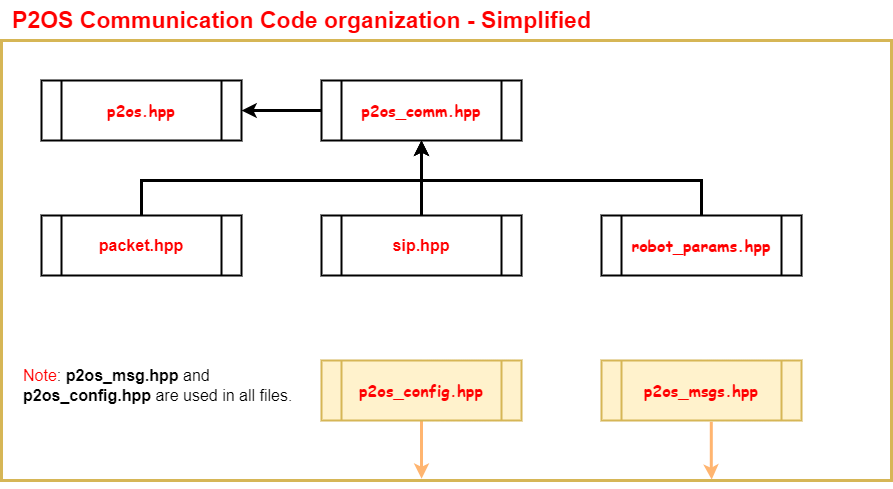
\includegraphics[width=15cm]{diagramas-test_setup-pioneer_2dx_interface-p2os_comm-simplified.drawio.png}
    \label{fig: Test Setup - P2OS Communication Code Organization - Simplified}
\end{figure}

\begin{itemize}
    \item \textbf{p2os}: Class responsible for performing the entire P2OS communication. It includes methods for startup, shutdown, handling main loop operations, retrieving robot data, and sending velocity and motor state formatted for the robot..
    \item \textbf{p2os\_comm}: Class responsible for encapsulating parameters, settings, and helper methods to perform the entire P2OS communication protocol correctly. This class is also responsible for managing the entire infinite state machine required to connect with the robot, as described in the topic \ref{P2OS - Communication protocol}.
    \item \textbf{packet}: Class responsible for building messages (adding headers and checksums), verifying received messages, receiving messages from the Pioneer 2DX, and sending messages to the Pioneer 2DX.
    \item \textbf{sip}: Class responsible for processing and managing data exchanged with a robot, such as separating the data into different types of variables and filtering out incorrect data.
    \item \textbf{robot\_params}: File responsible for managing all Pioneer robot type configurations, like the distance between wheels, available commands, number of ultrasonic sensors etc.
    \item \textbf{p2os\_config}: File responsible for maintaining all the P2OS protocol configurations.
    \item \textbf{p2os\_msgs}: File responsible for defining all message types used throughout the P2OS protocol.
\end{itemize}

As the \textbf{p2os.hpp} class describes the higher abstraction level of the communication, it is possible to observe in the main loop of this class how the algorithm works. Basically, every time the velocity input changes and it is a valid input value, it is sent to the robot, and the current data from the available sensors is retrieved. The same logic is applied to the motor state input. Additionally, at a predefined time interval specified in the \textbf{p2os\_config} file, a pulse is sent to the robot to maintain the connection. Furthermore, even if nothing is being sent, the SendReceive data function is called to continue receiving and saving data from the robot's sensors.

The main loop is described here in the code example \ref{lst:Part of the P2OS::loop() function}.

\begin{lstlisting}[
    language=C++,
    caption={Part of the P2OS::loop() function},
    label={lst:Part of the P2OS::loop() function},
]
void P2OS::loop() {
    this->current_time = millis();

    this->p2os_comm->check_and_set_vel();
    this->p2os_comm->check_and_set_motor_state();

    if (this->p2os_comm->get_pulse() > 0) {
        if (this->p2os_comm->millis2Sec(this->current_time - this->last_time_pulse) > this->p2os_comm->get_pulse()) {
#ifdef P2OS_DEBUG_PRINT
            this->debug_serial->println("sending pulse");
#endif
            this->p2os_comm->SendPulse();
            this->last_time_pulse = this->current_time;
        }
    }

    this->p2os_comm->SendReceive(NULL, true);
    this->p2os_comm->updateDiagnostics();
}
\end{lstlisting}


% \subsection{Bluepill test Firmware}

\end{document}

\begin{table}[h!]
\centering
\begin{tabular}{|c|c|c|}
\hline
\textbf{Pin Number} & \textbf{Esp32 Pin name} & \textbf{Label} \\ \hline
40 & GND  & gnd \\ \hline
39 & NC   & X \\ \hline
38 & SVN  & X \\ \hline
37 & IO35 & mode\_2 \\ \hline
36 & IO33 & mode\_1 \\ \hline
35 & IO34 & led\_conn\_esp \\ \hline
34 & TMS  & X \\ \hline
33 & NC   & encoder2\_s1 \\ \hline
32 & SD2  & encoder2\_s2 \\ \hline
31 & CMD  & encoder2\_s3 \\ \hline
30 & RST  & rst signal \\ \hline
29 & SVP  & dds\_8 \\ \hline
28 & IO26 & dds\_7 \\ \hline
27 & IO18 & dds\_6 \\ \hline
26 & IO19 & dds\_5 \\ \hline
25 & IO23 & dds\_4 \\ \hline
24 & IO5  & dds\_3 \\ \hline
23 & 3V3  & X \\ \hline
22 & TCK  & dds\_2 \\ \hline
21 & SD3  & dds\_1 \\ \hline
20 & TXD  & txd0\_micro \\ \hline
19 & RDX  & rxd0\_micro \\ \hline
18 & IO22 & X \\ \hline
17 & IO21 & X \\ \hline
16 & IO17 & txd2\_micro \\ \hline
15 & IO16 & rxd2\_micro \\ \hline
14 & GND  & gnd \\ \hline
13 & VCC  & 5v \\ \hline
12 & TD0  & X \\ \hline
11 & SD0  & p2dx\_con \\ \hline
10 & GND  & gnd \\ \hline
09 & IO27 & motor2\_comm1 \\ \hline
08 & IO25 & motor2\_comm2 \\ \hline
07 & IO32 & motor2\_comm3 \\ \hline
06 & TDI  & motor1\_comm1 \\ \hline
05 & IO4  & motor1\_comm2 \\ \hline
04 & IO0  & motor1\_comm3 \\ \hline
03 & IO2  & encoder1\_s3 \\ \hline
02 & SD1  & encoder1\_s2 \\ \hline
01 & CLK  & encoder1\_s1 \\ \hline
\end{tabular}
\caption{ESP32 Pin Mapping for Pioneer Communication}
\end{table}